\documentclass{math}

\usepackage{tikz}
\usetikzlibrary{quotes,angles}

\geometry{letterpaper, margin=1in}

\title{Section 7.3}
\author{Alvin Lin}
\date{Calculus II: August 2016 - December 2016}

\begin{document}

\maketitle

\section*{Exercise 9}
\[ \int_{2}^{3}{\frac{\diff{x}}{(x^{2}-1)^{\frac{3}{2}}}} \]
\[ Let: x = \sec(t) \]
\[ \diff{x} = \tan(t)\sec(t)\diff{t} \]
Solve as an indefinite integral:
\[ \int{\frac{1}{(\sec^{2}(t)-1)^{\frac{3}{2}}}\tan(t)\sec(t)\diff{t}} \]
\[ \int{\frac{\tan(t)\sec(t)}{(\tan^{2}(t))^{\frac{3}{2}}}\diff{t}} \]
\[ \int{\frac{\tan(t)\sec(t)}{\tan^{3}(t)}\diff{t}} \]
\[ \int{\frac{\sec(t)}{\tan^{2}(t)}\diff{t}} \]
\[ \int{\frac{1}{\cos(t)}\frac{\cos^{2}(t)}{\sin^{2}(t)}\diff{t}} \]
\[ \int{\cos(t)\sin^{-2}(t)\diff{t}} \]
\[ f(g(x)) = f'(g(x))g'(x) \]
\[ f'(x) = x^{-2} \quad g(x) = \sin(t) \quad g'(x) = \cos(t) \]
\[ Therefore: f(x) = \frac{-1}{x} \quad f(g(x)) = \frac{-1}{\sin(t)} \]
\[ \int{\cos(t)\sin^{-2}(t)\diff{t}} = \frac{-1}{\sin(t)}+C \]
Recall that we substituted \( x = \sec(t) \), which can be rewritten as
\( \sec(t) = \frac{x}{1} = \frac{hyp}{adj} \). If we imagine a triangle where
the hypotenuse is \( x \) and the adjacent side is 1, then the opposite side
must be \( \sqrt{x^{2}-1} \).
\begin{center}
  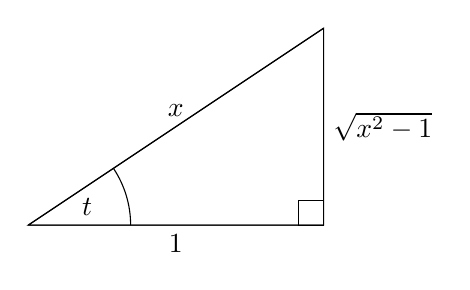
\begin{tikzpicture}[scale=1.25]
    \coordinate (A) at (-1.5cm,-1.0cm);
    \coordinate (B) at (1.5cm,1.0cm);
    \coordinate (C) at (1.5cm,-1.0cm);
    \draw (A)--node[above]{\( x \)}
          (B)--node[right]{\( \sqrt{x^{2}-1} \)}
          (C)--node[below]{\( 1 \)}(A);
    \draw (C) -- (A) -- (B) pic [draw,angle radius=13mm,"\( t \)"]
          {angle=C--A--B};
    \draw (1.25cm,-1.0cm) rectangle (1.5cm,-0.75cm);
  \end{tikzpicture}
\end{center}
Therefore: \( \sin(t) = \frac{opp}{hyp} = \frac{\sqrt{x^{2}-1}}{x} \)
\[ \frac{-1}{\sin(t)}+C = \frac{-x}{\sqrt{x^{2}-1}}+C \]
Now we integrate using the original limits:
\[ \bigg[\frac{-x}{\sqrt{x^{2}-1}}\bigg]_{2}^{3} \]
\[ (\frac{-3}{\sqrt{9-1}})-(\frac{-2}{\sqrt{4-1}}) \]
\[ \frac{-3}{2\sqrt{2}}+\frac{2}{\sqrt{3}} \]
\[ = \frac{2}{\sqrt{3}}-\frac{3}{2\sqrt{2}} \]

\section*{Exercise 19}
\[ \int{\frac{\sqrt{1+x^{2}}}{x}\diff{x}} \]
\[ Let: x = tan(t) \]
\[ \diff{x} = \sec^{2}(t)\diff{t} \]
\[ \int{\frac{\sqrt{1+\tan^{2}(t)}}{\tan(t)}\sec^{2}(t)\diff{t}} \]
\[ \int{\frac{\sqrt{\sec^{2}(t)}}{\tan(t)}\sec^{2}(t)\diff{t}} \]
\[ \int{\frac{\sec(t)}{\tan(t)}(\tan^{2}(t)+1)\diff{t}} \]
\[ \int{\sec(t)\tan(t)\diff{t}}+\int{\frac{\sec(t)}{\tan(t)}\diff{t}} \]
\[ \int{\sec(t)\tan(t)\diff{t}}+\int{\csc(t)}\diff{t} \]
\[ \sec^{2}(t)+\ln|\csc(t)-\cot(x)|+C \]
Recall that we substituted \( x=\tan(t) \), which can be rewritten as
\( \tan(t) = \frac{x}{1} = \frac{opp}{adj} \). If we imagine a triangle where
the opposide side is x and the adjacent side is 1, then the hypotenuse must be
\( \sqrt{1+x^{2}} \).
\begin{center}
  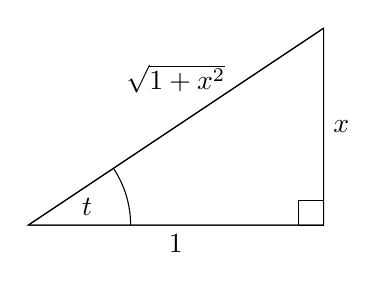
\begin{tikzpicture}[scale=1.25]
    \coordinate (A) at (-1.5cm,-1.0cm);
    \coordinate (B) at (1.5cm,1.0cm);
    \coordinate (C) at (1.5cm,-1.0cm);
    \draw (A)--node[above=0.3cm]{\( \sqrt{1+x^{2}} \)}
          (B)--node[right]{\( x \)}
          (C)--node[below]{\( 1 \)}(A);
    \draw (C) -- (A) -- (B) pic [draw,angle radius=13mm,"\( t \)"]
          {angle=C--A--B};
    \draw (1.25cm,-1.0cm) rectangle (1.5cm,-0.75cm);
  \end{tikzpicture}
\end{center}
Therefore:
\[ \sec(t) = \frac{hyp}{adj} = \sqrt{1+x^{2}} \]
\[ \csc(t) = \frac{hyp}{opp} = \frac{\sqrt{1+x^{2}}}{x} \]
\[ \cot(t) = \frac{adj}{opp} = \frac{1}{x} \]
\[ \sec^{2}(t)+\ln|\csc(t)-\cot(x)|+C = (\sqrt{1+x^{2}})^{2}+
   \ln\bigg|\frac{\sqrt{1+x^{2}}}{x}-\frac{1}{x}\bigg|+C \]
\[ = 1+x^{2}+\ln\bigg|\frac{\sqrt{1+x^{2}}-1}{x}\bigg|+C \]

\section*{Exercise 21}
\[ \int_{0}^{0.6}{\frac{x^{2}}{\sqrt{9-25x^{2}}}\diff{x}} \]
\[ Let: x = \frac{3}{5}\sin(t) \]
\[ \diff{x} = \frac{3}{5}\cos(t)\diff{t} \]
Solve as an indefinite integral:
\[ \int{\frac{\frac{9}{25}\sin^{2}(t)}{\sqrt{9-25(\frac{3}{5}\sin(t))^{2}}}
   \frac{3}{5}\cos(t)\diff{t}} \]
\[ \frac{27}{125}\int{\frac{\sin^{2}(t)}
   {\sqrt{9}\sqrt{1-\sin^{2}(t)}}\cos(t)\diff{t}} \]
\[ \frac{9}{125}\int{\frac{\sin^{2}(t)}{\sqrt{\cos^{2}(t)}}\cos(t)\diff{t}} \]
\[ \frac{9}{125}\int{\sin^{2}(t)\diff{t}} \]
\[ \frac{9}{125}\int{\frac{1-\cos(2t)}{2}\diff{t}} \]
\[ \frac{9}{250}\int{1-\cos(2t)\diff{t}} \]
\[ \frac{9}{250}\bigg(\int{1\diff{t}}-\int{\cos(2t)\diff{t}}\bigg) \]
\[ \frac{9}{250}\bigg(t-\frac{1}{2}\sin(2t)\bigg)+C \]
\[ \frac{9}{250}\bigg(t-\frac{1}{2}2\sin(t)\cos(t)\bigg)+C \]
\[ \frac{9}{250}\bigg(t-\sin(t)\cos(t)\bigg)+C \]
Recall that we substituted \( x = \frac{3}{5}\sin(t) \), which can be rewritten
as \( \sin(t) = \frac{5x}{3} = \frac{opp}{hyp} \). If we imagine a triangle
where the opposide side is \( 5x \) and the hypotenuse is 3, then the adjacent
side must be \( \sqrt{9-25x^{2}} \).
\begin{center}
  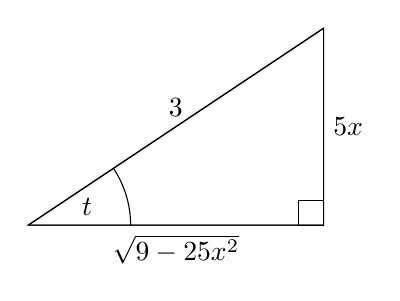
\begin{tikzpicture}[scale=1.25]
    \coordinate (A) at (-1.5cm,-1.0cm);
    \coordinate (B) at (1.5cm,1.0cm);
    \coordinate (C) at (1.5cm,-1.0cm);
    \draw (A)--node[above]{\( 3 \)}
          (B)--node[right]{\( 5x \)}
          (C)--node[below]{\( \sqrt{9-25x^{2}} \)}(A);
    \draw (C) -- (A) -- (B) pic [draw,angle radius=13mm,"\( t \)"]
          {angle=C--A--B};
    \draw (1.25cm,-1.0cm) rectangle (1.5cm,-0.75cm);
  \end{tikzpicture}
\end{center}
Therefore:
\[ \cos(t) = \frac{\sqrt{9-25x^{2}}}{3} \]
\[ t = \arcsin(\frac{5x}{3}) \]
\[ \frac{9}{250}\bigg(t-\sin(t)\cos(t)\bigg)+C =
   \frac{9}{250}\bigg(\arcsin(\frac{5x}{3})-
   \frac{5x}{3}\frac{\sqrt{9-25x^{2}}}{3}\bigg)+C \]
\[ \frac{9\arcsin(\frac{5x}{3})}{250}-\frac{5x\sqrt{9-25x^{2}}}{250}+C \]
Now we integrate using the original limits:
\[ \bigg[\frac{9\arcsin(\frac{5x}{3})}{250}-
   \frac{5x\sqrt{9-25x^{2}}}{250}\bigg]_{0}^{0.6} \]
\[ \bigg[\frac{9\arcsin(\frac{3}{3})}{250}-\frac{3\sqrt{9-9}}{250}\bigg]-
   \bigg[\frac{9\arcsin(\frac{0}{3})}{250}-\frac{0\sqrt{9-0}}{250}\bigg] \]
\[ \bigg[\frac{9\frac{\pi}{2}}{250}-0\bigg]-0 \]
\[ = \frac{9\pi}{500} \]

\section*{Exercise 23}
\[ \int{\frac{\diff{x}}{x^{2}+2x+5}} \]
\[ \int{\frac{\diff{x}}{x^{2}+2x+1+4}} \]
\[ \int{\frac{\diff{x}}{(x+1)^{2}+4}} \]
\[ Let: x+1 = 2\tan(t) \]
\[ \diff{x} = 2\sec^{2}(t)\diff{t} \]
\[ \int{\frac{2\sec^{2}(t)}{(2\tan(t))^{2}+4}\diff{t}} \]
\[ \int{\frac{2\sec^{2}(t)}{4\tan^{2}(t)+4}\diff{t}} \]
\[ \frac{1}{2}\int{\frac{\sec^{2}(t)}{\tan^{2}(t)+1}\diff{t}} \]
\[ \frac{1}{2}\int{\frac{\sec^{2}(t)}{\sec^{2}(t)}\diff{t}} \]
\[ \frac{1}{2}\int{1\diff{t}} \]
\[ \frac{1}{2}t+C \]
Given our original substitution \( x+1 = 2\tan(t) \), we can rewrite this as
\( \tan(t) = \frac{x+1}{2} \) and get the equation
\( \arctan(\frac{x+1}{2}) = t \).
Therefore:
\[ \frac{1}{2}t+C = \frac{\arctan(\frac{x+1}{2})}{2}+C \]

\begin{center}
  If you have any questions, comments, or concerns, please contact me at
  alvin@omgimanerd.tech
\end{center}

\end{document}
